\documentclass{standalone}
\usepackage{pgf, tikz}
\usepackage{mathtools}
\usetikzlibrary{arrows, automata}

\begin{document}

    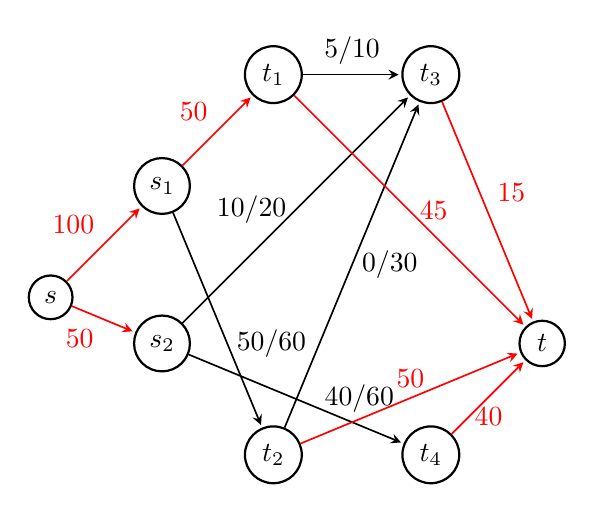
\begin{tikzpicture}[
            > = stealth, % arrow head style
            shorten > = 1pt, % don't touch arrow head to node set to +pt
            auto,
            node distance = 2cm, % distance between nodes
            semithick % line style
        ]

        \tikzstyle{every state}=[
            draw = black,
            thick,
            fill = white,
            minimum size = 2mm
        ]

        \node[state] (s) {$s$};
        \node[state] (s1) [above right of=s] {$s_1$};
        \node[state] (s2) [below of=s1] {$s_2$};
        \node[state] (t1) [above right of=s1] {$t_1$};
        \node[state] (t2) [below right of=s2] {$t_2$};
        \node[state] (t3) [right of=t1] {$t_3$};
        \node[state] (t4) [right of=t2] {$t_4$};
        \node[state] (t) [above right of=t4] {$t$};


        \path[->, color=red] (s) edge node {$100$} (s1);
        \path[->,color=red] (s) edge node[below left] {$50$} (s2);
        \path[->, color=red] (s1) edge node[above left] {$50$} (t1);
        \path[->] (s1) edge node[below right] {$~50/60$} (t2);
        \path[->] (s2) edge node[left] {$10/20$} (t3);
        \path[->] (s2) edge node[right] {$~~40/60$} (t4);
        \path[->] (t2) edge node[right] {$0/30$} (t3);
        \path[->] (t1) edge node {$5/10$} (t3);
        \path[->, color=red] (t1) edge node[right] {$45$} (t);
        \path[->, color=red] (t2) edge node[above] {$50$} (t);
        \path[->, color=red] (t3) edge node {$15$} (t);
        \path[->, color=red] (t4) edge node[below] {$40$} (t);

    \end{tikzpicture}

\end{document}
